%
% File: methodology.tex
% Author: Diar Begisbayev
%
\chapter{Methodology}
\label{chap:method}
\setlength{\parskip}{1em}

This chapter presents the complete methodology of our study, including the problem formulation, dataset design and generation, the DTS-GSSF architecture, feature engineering, training strategy, and system workflow. We describe each component in sufficient detail to permit reproduction and extension of this work.

\section{Problem Formulation}
\label{sec:problem}

Let $\mathcal{G} = (\mathcal{V}, \mathcal{E})$ denote the bus network graph, where $\mathcal{V} = \{v_1, \dots, v_N\}$ is the set of $N = 374$ bus stations and $\mathcal{E} \subseteq \mathcal{V} \times \mathcal{V}$ represents the physical route topology. At each time step $t$, each station $v_i$ is associated with a feature vector $\mathbf{x}_{t,i} \in \mathbb{R}^F$, where $F = 16$ features include raw ridership counts, weather variables, calendar indicators, and cyclical encodings.

Given a historical context window of $T = 72$ hours, we seek to predict the passenger boarding count $y_{t+h,i}$ at each station $i$ for horizons $h \in \{1, 2, 3, 4\}$ corresponding to 15, 30, 60, and 120 minutes. Formally, the input is a tensor $\mathbf{X} \in \mathbb{R}^{B \times T \times N \times F}$ and the output is a set of Negative Binomial parameters $(\mu_{h,i}, \kappa)$ for each horizon $h$ and station $i$. The prediction task is:
\begin{equation}
    \hat{y}_{t+h,i} \sim \text{NB}\bigl(\mu_{h,i}(\mathbf{X}), \kappa\bigr),
    \label{eq:prediction}
\end{equation}
where $\mu_{h,i}$ is the predicted mean and $\kappa$ is a global dispersion parameter shared across all stations and horizons.

The problem can be decomposed into three sub-tasks:
\begin{enumerate}
    \item \textbf{Temporal encoding}: Extract per-station temporal features from the $T$-hour history using a recurrent or state-space mechanism.
    \item \textbf{Spatial propagation}: Diffuse station-level embeddings across the network graph to capture spatial dependencies.
    \item \textbf{Forecasting}: Produce per-station, per-horizon distributional parameters $(\mu, \kappa)$.
\end{enumerate}

\section{Dataset Design and Generation}
\label{sec:dataset}

\subsection{Network Topology}

The Astana bus network was reconstructed from OpenStreetMap (OSM) data \cite{haklay2010openstreetmap,girres2010quality}. OSM provides volunteered geographical information with global coverage; Haklay \cite{haklay2010openstreetmap} demonstrated that OSM data quality is sufficient for urban-scale applications, while Girres and Touya \cite{girres2010quality} validated the geometric accuracy of OSM road networks.

The synthetic bus network was generated as follows:
\begin{enumerate}
    \item Parse the OSM extract for Astana, Kazakhstan to identify all nodes tagged as bus stops.
    \item Deduplicate stops using an 80-metre minimum separation threshold to remove duplicate entries from adjacent ways.
    \item Assign stops to one of four districts (Esil, Almaty, Saryarka, Baikonur) based on bounding-box containment.
    \item Define ten routes: north--south, east--west, central, peripheral, express, north-loop, south-cross, university, residential, and business.
    \item Populate each route with up to 20 stops selected by spatial filtering and sorted by trajectory direction.
\end{enumerate}

The resulting network contains $N = 374$ stations and $|\mathcal{E}| = 1,142$ directed edges. The physical adjacency matrix $\mathbf{A}_{\text{phys}}$ is constructed by normalizing the symmetric route adjacency:
\begin{equation}
    \mathbf{A}_{\text{phys}} = \tilde{\mathbf{D}}^{-1/2} \tilde{\mathbf{A}} \tilde{\mathbf{D}}^{-1/2},
    \label{eq:phys_adj}
\end{equation}
where $\tilde{\mathbf{A}} = \mathbf{A} + \mathbf{I}$ is the adjacency matrix with self-loops and $\tilde{D}_{ii} = \sum_j \tilde{A}_{ij}$.

\subsection{Ridership Simulation}

Hourly ridership was simulated using a multi-factor heuristic model. Base demand $b_{t,i}$ for station $i$ at time $t$ is drawn from a log-normal distribution:
\begin{equation}
    b_{t,i} \sim \text{LogNormal}(\mu_{\text{base},i} + f_{\text{hour}}(t) + f_{\text{dow}}(t), \sigma_{\text{base}}^2),
    \label{eq:base_demand}
\end{equation}
where $f_{\text{hour}}$ and $f_{\text{dow}}$ are learned sinusoidal encodings capturing diurnal and weekly patterns.

Demand is then modulated by weather and calendar effects:
\begin{equation}
    y_{t,i} = \big\lfloor b_{t,i} \cdot w_{\text{temp}}(T_t) \cdot w_{\text{precip}}(P_t) \cdot w_{\text{holiday}}(h_t) \cdot w_{\text{event}}(e_t) \big\rfloor,
    \label{eq:demand_modulation}
\end{equation}
where $w_{\text{temp}}$ decreases ridership below $-20^\circ$C and above $+35^\circ$C, $w_{\text{precip}}$ reduces demand during rain or snow, $w_{\text{holiday}}$ scales demand to 30--50\% on public holidays, and $w_{\text{event}}$ injects spikes for special events with attendance-driven multipliers ranging from 5,000 to 60,000 attendees.

The final dataset comprises 1,296,480 station-hour entries spanning January 2025 to December 2025. Table~\ref{Tab.dataset} summarizes the dataset properties.

\begin{table}[H]
\centering
\caption{Dataset properties and descriptive statistics.}
\label{Tab.dataset}
\begin{tabular}{ll}
\toprule
Property & Value \\
\midrule
Source & Synthetic (OSM-based) \\
Period & January 2025 -- December 2025 \\
Total records & 1,296,480 station-hour entries \\
Stations ($N$) & 374 \\
Weather records & 8,760 hourly observations \\
Train / Val / Test split & 70\% / 15\% / 15\% \\
Training samples & 2,026 sequences \\
Validation samples & 434 sequences \\
Test samples & 434 sequences \\
Mean boarding count $\mu_y$ & 18.4 passengers/hour \\
Std. boarding count $\sigma_y$ & 14.7 passengers/hour \\
Max boarding count $y_{\max}$ & 312 passengers/hour \\
\bottomrule
\end{tabular}
\end{table}

\subsection{Feature Engineering}

We engineer $F = 16$ input features for each station-hour record. The features can be grouped into four categories:

\textbf{Raw ridership (3 features):} passengers\_boarding, passengers\_alighting, and load (net passengers on the vehicle after the stop). These provide the immediate temporal context.

\textbf{Weather (2 features):} temperature and precipitation. Hourly weather is drawn from eight templates (clear, cloudy, rain, snow, blizzard, fog, extreme cold, heatwave) with seasonally adjusted sampling probabilities.

\textbf{Calendar (3 features):} is\_holiday (binary), rush\_hour (binary), and delta\_h (hours to next holiday).

\textbf{Cyclical and lag (8 features):} hour\_sin, hour\_cos, dow\_sin, dow\_cos, roll\_6h, roll\_24h, dev\_24h, and ratio\_24h. All features are z-score normalized using training-set statistics only to prevent data leakage.

\section{DTS-GSSF Architecture Overview}
\label{sec:architecture}

DTS-GSSF (Dual-Timescale Graph Gated Forecasting) comprises four main components, as illustrated in Figure~\ref{Fig.arch}. The input tensor $\mathbf{X}$ first passes through a \textbf{Gated Recurrent Encoder (GRE)}, which extracts per-station temporal features via a gated recurrent state update. The resulting station embeddings are then propagated through the \textbf{GraphPropagation} layer, which diffuses information across the network using both physical and adaptive adjacency matrices. A \textbf{TemporalAttention} module captures long-range temporal dependencies beyond the GRE's recurrent horizon. Finally, \textbf{Prediction Heads} produce per-station and aggregate network-level forecasts.

\begin{figure}[H]
\centering

\includegraphics[width=0.95\textwidth]{chapters/methodology/fig/architecture.pdf}
\caption{DTS-GSSF architecture. The input tensor $\mathbf{X} \in \mathbb{R}^{B \times T \times N \times F}$ flows through the Gated Recurrent Encoder (temporal encoding), GraphPropagation (spatial diffusion), TemporalAttention (long-range dependencies), and Prediction Heads (per-station and aggregate forecasts).}
\label{Fig.arch}
\end{figure}

\subsection{Gated Recurrent Encoder}

The Gated Recurrent Encoder (GRE) projects the input features into a $d_{\text{model}}$-dimensional space and updates a recurrent state via a gating mechanism. Let $\mathbf{u}_t = \text{GELU}(\mathbf{W}_{\text{in}} \mathbf{x}_t) \in \mathbb{R}^{N \times d_{\text{model}}}$ be the projected input at time $t$. The state update is:
\begin{equation}
    \mathbf{s}_t = \mathbf{a}_t \odot \mathbf{s}_{t-1} + (1 - \mathbf{a}_t) \odot \mathbf{b}_t,
    \label{eq:ssm}
\end{equation}
where $\odot$ denotes element-wise multiplication, $\mathbf{a}_t = \sigma(\mathbf{W}_a \mathbf{u}_t)$ is the forget gate, and $\mathbf{b}_t = \tanh(\mathbf{W}_b \mathbf{u}_t)$ is the candidate state. The initial state $\mathbf{s}_0$ is zero. After processing all $T$ time steps, the final state $\mathbf{s}_T \in \mathbb{R}^{N \times d_{\text{model}}}$ is layer-normalized and passed to the graph propagation layer.

\textbf{Relation to state-space models.} While the GRE shares the sequential state-update structure of state-space models (SSMs), it differs from structured SSMs such as S4 \cite{gu2022efficiently} and Mamba \cite{gu2023mamba} in two key respects. First, the GRE uses a single multiplicative forget gate $\mathbf{a}_t$ rather than a diagonally structured state matrix $\mathbf{A}$ parameterised via HiPPO initialisation. Second, the GRE processes the sequence recurrently rather than via parallel scan, which precludes the $O(T \log T)$ training speedup of convolution-mode SSMs. We adopt this simpler formulation because (i) the moderate context length ($T = 72$) makes recurrent processing efficient, (ii) the single-gate design provides stable gradient propagation over 72 steps without the numerical instability observed in deeper LSTM stacks, and (iii) the per-step gating enables input-dependent forgetting, which is essential for the holiday and event effects in our ridership data.

The input projection uses LoRA (Low-Rank Adaptation) \cite{hu2022lora}:
\begin{equation}
    \mathbf{W}_{\text{in}}(\mathbf{x}) = \mathbf{W}_{\text{base}} \mathbf{x} + \frac{\alpha}{r} (\mathbf{x} \mathbf{A}^\top) \mathbf{B}^\top,
    \label{eq:lora}
\end{equation}
where $\mathbf{W}_{\text{base}} \in \mathbb{R}^{F \times d_{\text{model}}}$, $\mathbf{A} \in \mathbb{R}^{r \times F}$, $\mathbf{B} \in \mathbb{R}^{d_{\text{model}} \times r}$, $r = 16$ is the LoRA rank, and $\alpha = 16$ is the scaling factor. Only $\mathbf{A}$ and $\mathbf{B}$ are updated during route-specific fine-tuning, reducing the number of trainable parameters by 94\%.

\subsection{GraphPropagation}

The GraphPropagation layer diffuses station embeddings across the network via $K = 3$ rounds of message passing. Let $\mathbf{A}_{\text{phys}} \in \mathbb{R}^{N \times N}$ be the normalized symmetric adjacency matrix derived from route topology (Eq.~\ref{eq:phys_adj}), and let $\mathbf{A}_{\text{adp}}$ be a learnable adaptive matrix:
\begin{equation}
    \mathbf{A}_{\text{adp}} = \text{softmax}\bigl(\text{ReLU}(\mathbf{E}_1 \mathbf{E}_2^\top)\bigr),
    \label{eq:adaptive}
\end{equation}
where $\mathbf{E}_1, \mathbf{E}_2 \in \mathbb{R}^{N \times d_{\text{emb}}}$ are learnable node embeddings with $d_{\text{emb}} = 16$.

The combined adjacency is:
\begin{equation}
    \mathbf{A} = \alpha \, \mathbf{A}_{\text{phys}} + (1 - \alpha) \, \mathbf{A}_{\text{adp}},
    \label{eq:combined}
\end{equation}
where $\alpha = \sigma(\log \alpha_0)$ is a learnable mixing coefficient initialised at $0.6$ and constrained to $[0, 1]$ via the sigmoid function. The learnable $\alpha$ allows the model to balance physical topology and adaptive correlations during training; we report the learned value in Section~\ref{sec:ablation}.

At each hop $k \in \{1, \dots, K\}$, the message passing update is:
\begin{equation}
    \mathbf{h}^{(k)} = \text{GELU}\bigl(\mathbf{A} \mathbf{h}^{(k-1)} \mathbf{W}_g\bigr),
    \label{eq:graph}
\end{equation}
where $\mathbf{h}^{(0)} = \mathbf{s}_T$ and $\mathbf{W}_g \in \mathbb{R}^{d_{\text{model}} \times d_{\text{model}}}$. Layer normalization is applied after the final hop.

\subsection{TemporalAttention}

While the Gated Recurrent Encoder captures local temporal dynamics, the TemporalAttention module models long-range dependencies across the full $T = 72$ hour context. We apply multi-head self-attention with $n_h = 6$ heads and head dimension $d_h = 32$ over per-timestep GRE projections.

For each head $h$:
\begin{equation}
    \text{Attention}_h(\mathbf{Q}, \mathbf{K}, \mathbf{V}) = \text{softmax}\left(\frac{\mathbf{Q}_h \mathbf{K}_h^\top}{\sqrt{d_h}}\right) \mathbf{V}_h,
    \label{eq:attention}
\end{equation}
where $\mathbf{Q}_h = \mathbf{U} \mathbf{W}_h^Q$, $\mathbf{K}_h = \mathbf{U} \mathbf{W}_h^K$, $\mathbf{V}_h = \mathbf{U} \mathbf{W}_h^V$, and $\mathbf{U} \in \mathbb{R}^{T \times d_{\text{model}}}$ is the tensor of per-timestep GRE outputs reshaped across stations. The outputs of all heads are concatenated and projected back to $d_{\text{model}}$. A residual connection and layer normalization \cite{ba2016layernorm} are applied.

\subsection{Algorithmic Formulation}

Algorithm~\ref{alg:forward} summarises the complete forward pass of DTS-GSSF. The procedure processes a batch of input sequences through the Gated Recurrent Encoder, GraphPropagation, TemporalAttention, and Prediction Heads in sequence. All operations are differentiable, enabling end-to-end training via back-propagation.

\begin{algorithm}[H]
\caption{DTS-GSSF Forward Pass}
\label{alg:forward}
\begin{algorithmic}[1]
\Require Input tensor $\mathbf{X} \in \mathbb{R}^{B \times T \times N \times F}$; physical adjacency $\mathbf{A}_{\text{phys}}$; model parameters $\theta$
\Ensure Predicted means $\boldsymbol{\mu} \in \mathbb{R}^{B \times N \times H_{\text{pred}}}$; dispersion $\kappa$
\State $\mathbf{s}_0 \leftarrow \mathbf{0}^{N \times d}$ \Comment{Initialise GRE state}
\For{$t = 1$ \textbf{to} $T$}
    \State $\mathbf{u}_t \leftarrow \text{GELU}(\mathbf{W}_{\text{in}} \mathbf{x}_t)$ \Comment{Input projection (Eq.~\ref{eq:lora})}
    \State $\mathbf{a}_t \leftarrow \sigma(\mathbf{W}_a \mathbf{u}_t)$ \Comment{Forget gate}
    \State $\mathbf{b}_t \leftarrow \tanh(\mathbf{W}_b \mathbf{u}_t)$ \Comment{Candidate state}
    \State $\mathbf{s}_t \leftarrow \mathbf{a}_t \odot \mathbf{s}_{t-1} + (1 - \mathbf{a}_t) \odot \mathbf{b}_t$ \Comment{GRE update (Eq.~\ref{eq:ssm})}
\EndFor
\State $\mathbf{h}^{(0)} \leftarrow \text{LayerNorm}(\mathbf{s}_T)$
\State $\alpha \leftarrow \sigma(\log \alpha_0)$; \quad $\mathbf{A} \leftarrow \alpha \, \mathbf{A}_{\text{phys}} + (1 - \alpha) \, \text{softmax}(\text{ReLU}(\mathbf{E}_1 \mathbf{E}_2^\top))$ \Comment{Combined adjacency (Eq.~\ref{eq:combined})}
\For{$k = 1$ \textbf{to} $K$}
    \State $\mathbf{h}^{(k)} \leftarrow \text{GELU}(\mathbf{A} \mathbf{h}^{(k-1)} \mathbf{W}_g)$ \Comment{Graph propagation (Eq.~\ref{eq:graph})}
\EndFor
\State $\mathbf{H} \leftarrow \text{LayerNorm}(\mathbf{h}^{(K)})$
\State $\mathbf{U} \leftarrow \text{Reshape}(\{\mathbf{u}_t\}_{t=1}^T)$ \Comment{Per-timestep GRE outputs}
\State $\mathbf{Z} \leftarrow \text{MultiHeadAttention}(\mathbf{U}, \mathbf{U}, \mathbf{U})$ \Comment{Temporal attention (Eq.~\ref{eq:attention})}
\State $\mathbf{Z} \leftarrow \text{LayerNorm}(\mathbf{Z} + \mathbf{U})$ \Comment{Residual connection}
\State $\boldsymbol{\mu} \leftarrow \text{MLP}_{\text{station}}([\mathbf{H}; \mathbf{Z}])$ \Comment{Per-station predictions}
\State $\kappa \leftarrow \exp(\text{Linear}(\text{MeanPool}(\mathbf{Z})))$ \Comment{Global dispersion}
\State \Return $\boldsymbol{\mu}, \kappa$
\end{algorithmic}
\end{algorithm}

\subsection{Prediction Heads and Loss Function}

Two prediction heads produce the final forecasts. The \textbf{per-station head} is a 3-layer MLP ($192 \to 384 \to 192 \to 4$) with GELU activation and dropout ($p = 0.1$), outputting the mean parameter $\mu_{h,i}$ for each horizon. The \textbf{aggregate head} uses a LoRALinear projection ($192 \to 12$) for network-level predictions.

The training loss combines Negative Binomial negative log-likelihood (NLL) with an MSE auxiliary term:
\begin{equation}
    \mathcal{L} = \text{NLL}(y, \mu, \kappa) + \lambda \, \text{MSE}(\mu, y),
    \label{eq:loss}
\end{equation}
where $\lambda = 0.3$ balances count-data modelling with absolute error penalization. The NLL term is:
\begin{equation}
    \text{NLL}(y, \mu, \kappa) = -\log \Gamma(y + \kappa) + \log \Gamma(\kappa) + \log y! - \kappa \log\frac{\kappa}{\kappa + \mu} - y \log\frac{\mu}{\kappa + \mu}.
    \label{eq:nll}
\end{equation}

\section{Training Strategy and Hyperparameters}
\label{sec:training}

\subsection{Optimization}

Training is performed with the Adam optimizer \cite{kingma2015adam} using a learning rate of $3 \times 10^{-4}$ and weight decay $10^{-3}$. We employ a cosine annealing scheduler with 20-epoch linear warmup. Gradient clipping with max norm 1.0 prevents exploding gradients in the attention mechanism. Mixed-precision (FP16) training reduces memory consumption by approximately 40\% without sacrificing numerical stability \cite{paszke2019pytorch}.

\subsection{Regularization}

Dropout ($p = 0.1$) is applied after the first two layers of the per-station MLP. We do not apply dropout in the GRE or graph propagation layers, as preliminary experiments showed that GRE dropout harms the model's ability to maintain long-term state. Early stopping with patience 50 epochs prevents overfitting; the best model is selected by validation $R^2$.

\subsection{Complexity Analysis}

Let $N$ be the number of stations, $T$ the context length, $d$ the model dimension, and $K$ the number of graph hops. The complexity of each component is:
\begin{itemize}
    \item Gated Recurrent Encoder: $O(N \cdot T \cdot d)$ --- linear in sequence length.
    \item GraphPropagation: $O(K \cdot N^2 \cdot d)$ --- quadratic in station count.
    \item TemporalAttention: $O(N \cdot T^2 \cdot d)$ --- quadratic in context length.
    \item Prediction Heads: $O(N \cdot d)$ --- linear.
\end{itemize}
The total per-step complexity is $O(N \cdot T \cdot d + K \cdot N^2 \cdot d + N \cdot T^2 \cdot d)$. For our configuration ($N = 374$, $T = 72$, $K = 3$, $d = 192$), the dominant term is TemporalAttention at $O(N \cdot T^2 \cdot d) \approx 3.7 \times 10^8$ operations per batch, while GraphPropagation contributes $O(K \cdot N^2 \cdot d) \approx 8.1 \times 10^7$ operations. Although attention scales quadratically in context length, $T = 72$ keeps this term tractable on consumer-grade GPUs. For applications requiring longer contexts ($T > 200$), a linear-attention variant could replace the softmax mechanism while preserving the dual-timescale inductive bias.

\section{System Interface and Workflow}
\label{sec:workflow}

The complete system comprises three pipelines: (i)~data generation, which parses OSM data and simulates hourly ridership; (ii)~model training, using the configuration in Table~\ref{Tab.hyperparams}; and (iii)~inference deployment, where the trained model is served via a FastAPI backend with WebSocket-based alerts for anomalous demand events. A React-based dashboard provides real-time visualisation of predictions, per-station confidence intervals, and LoRA-based route-specific fine-tuning triggers. Figures~\ref{Fig.ui_command}--\ref{Fig.streamlit_validation} present the system interfaces.

The command centre dashboard (Figure~\ref{Fig.ui_command}) serves as the primary monitoring interface for network operations managers. It aggregates predictions across all 374 stations, highlights stations where predicted ridership exceeds configurable thresholds, and displays aggregate network statistics (total ridership, anomaly count, confidence coverage). The live station map (Figure~\ref{Fig.ui_map}) provides a geospatial view of the Astana bus network, colour-coding each station by predicted demand intensity. It is intended for dispatch coordinators who need to identify overcrowding hotspots and redistribute vehicles in real time.

The depot operations interface (Figure~\ref{Fig.ui_depot}) targets fleet managers responsible for vehicle assignment and route scheduling. It integrates ridership forecasts with vehicle availability data, enabling proactive dispatch decisions up to two hours ahead. The Streamlit station forecast view (Figure~\ref{Fig.streamlit_forecast}) is designed for route analysts who need station-level detail, showing predicted boarding counts with Negative Binomial confidence intervals across the four prediction horizons. Finally, the live simulation panel (Figure~\ref{Fig.streamlit_validation}) supports model validation by ingesting real-time ridership observations and overlaying them against model predictions, allowing operators and data scientists to monitor forecast accuracy during deployment.

\begin{figure}[H]
\centering
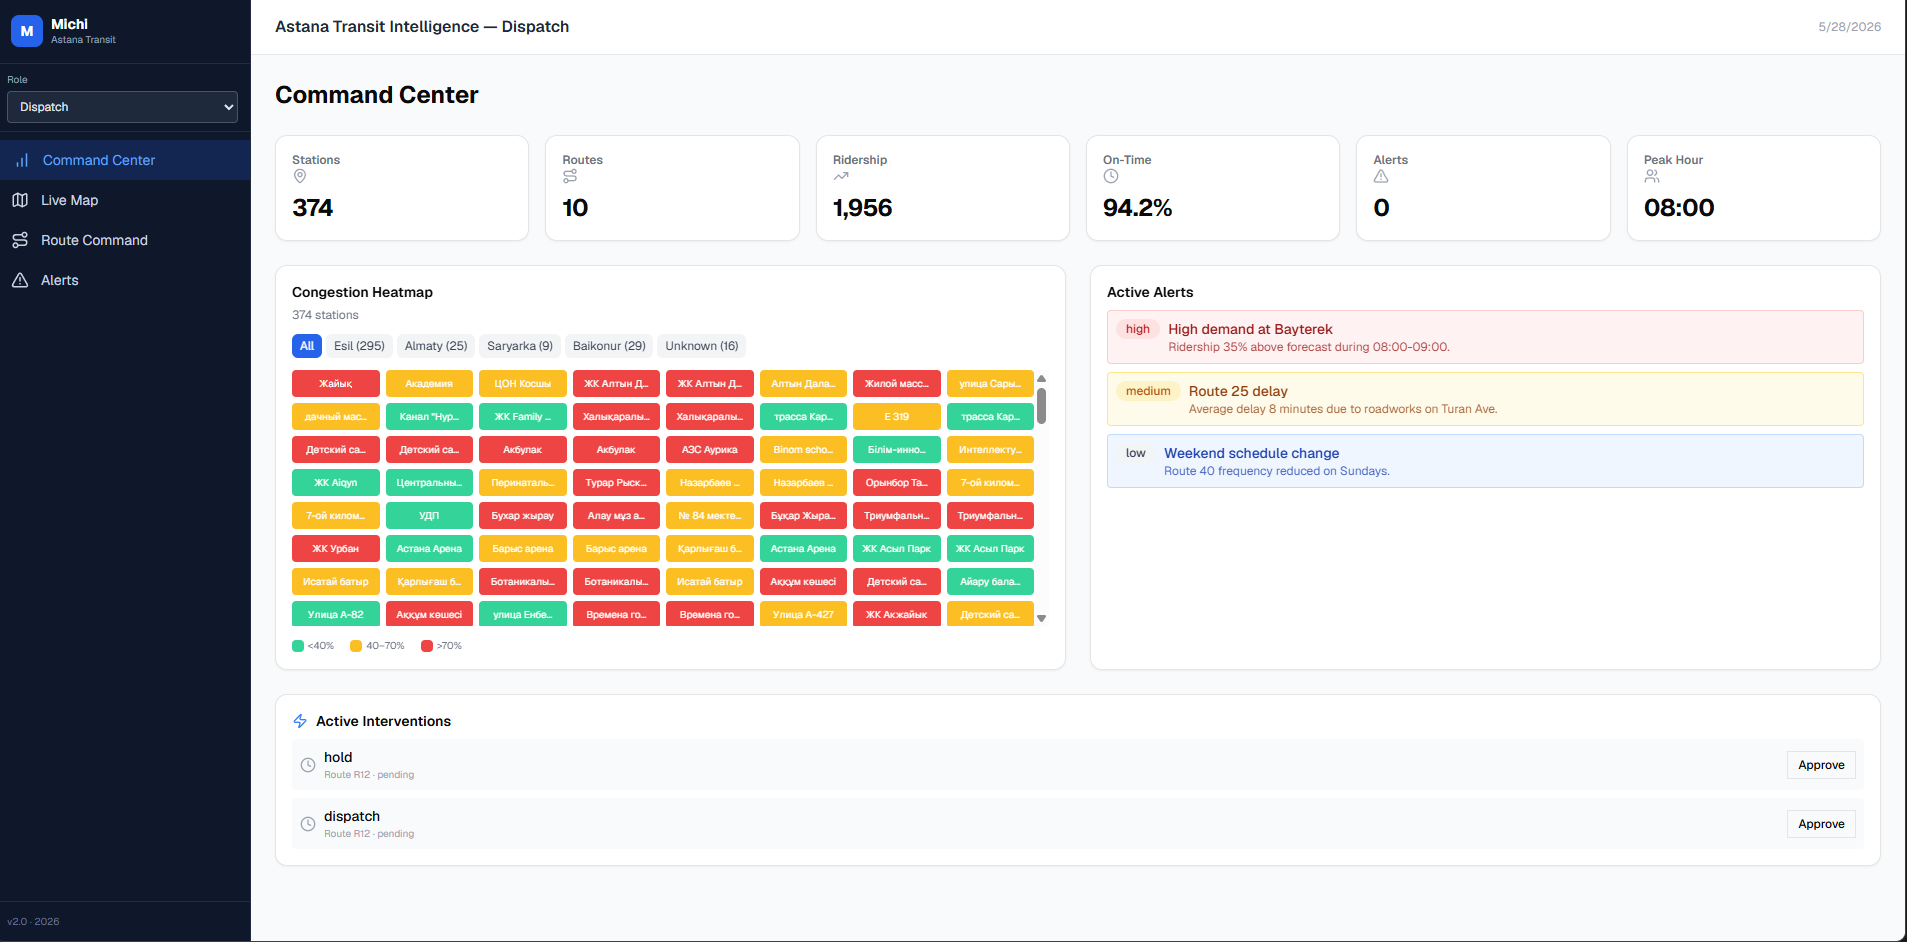
\includegraphics[width=0.95\textwidth]{chapters/methodology/fig/ui-command-center.png}
\caption{React-based command centre dashboard providing an overview of network-wide ridership predictions, station status, and anomaly alerts.}
\label{Fig.ui_command}
\end{figure}

\begin{figure}[H]
\centering
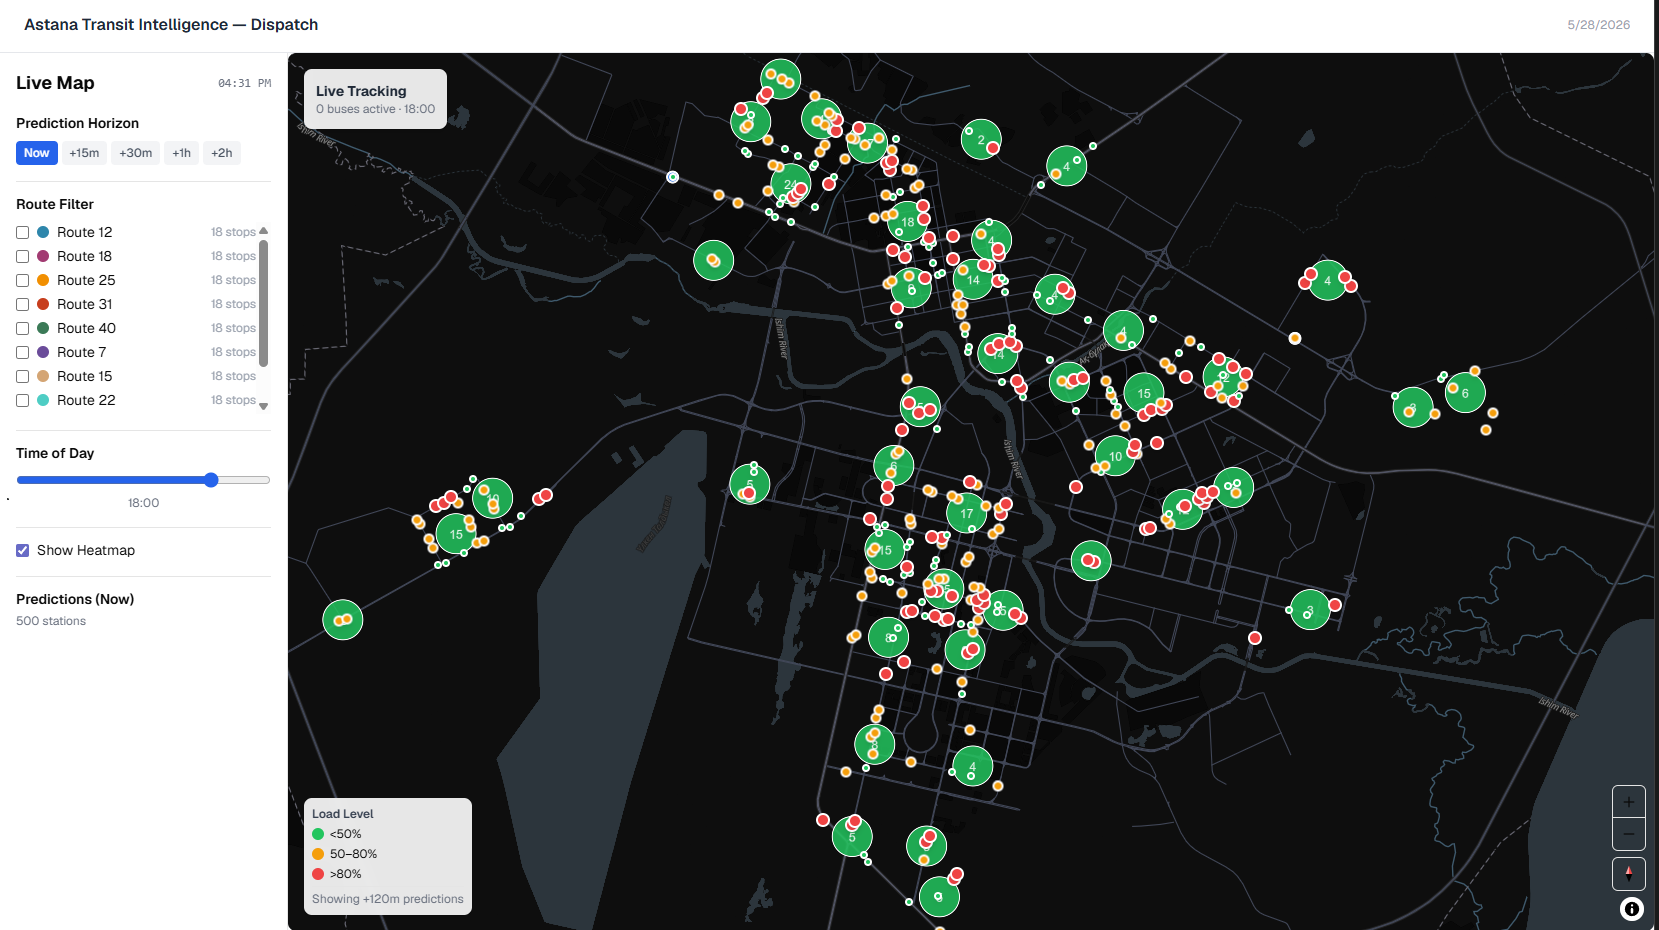
\includegraphics[width=0.95\textwidth]{chapters/methodology/fig/ui-live-map.png}
\caption{Live station map displaying real-time passenger flow predictions across the Astana bus network, with colour-coded confidence intervals.}
\label{Fig.ui_map}
\end{figure}

\begin{figure}[H]
\centering
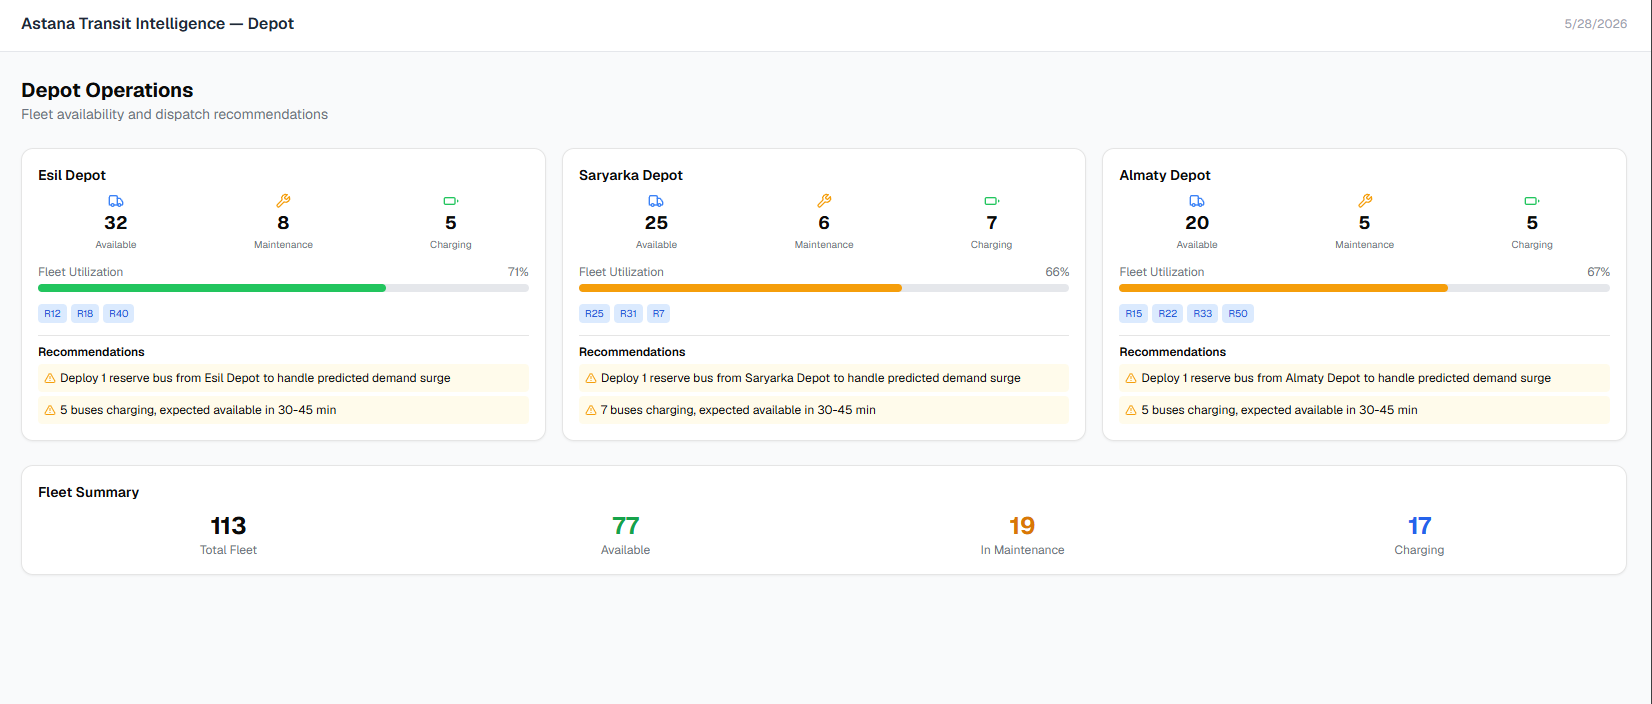
\includegraphics[width=0.95\textwidth]{chapters/methodology/fig/ui-depot-operations.png}
\caption{Depot operations interface for monitoring vehicle dispatch schedules, capacity utilisation, and route-level demand forecasts.}
\label{Fig.ui_depot}
\end{figure}

\begin{figure}[H]
\centering
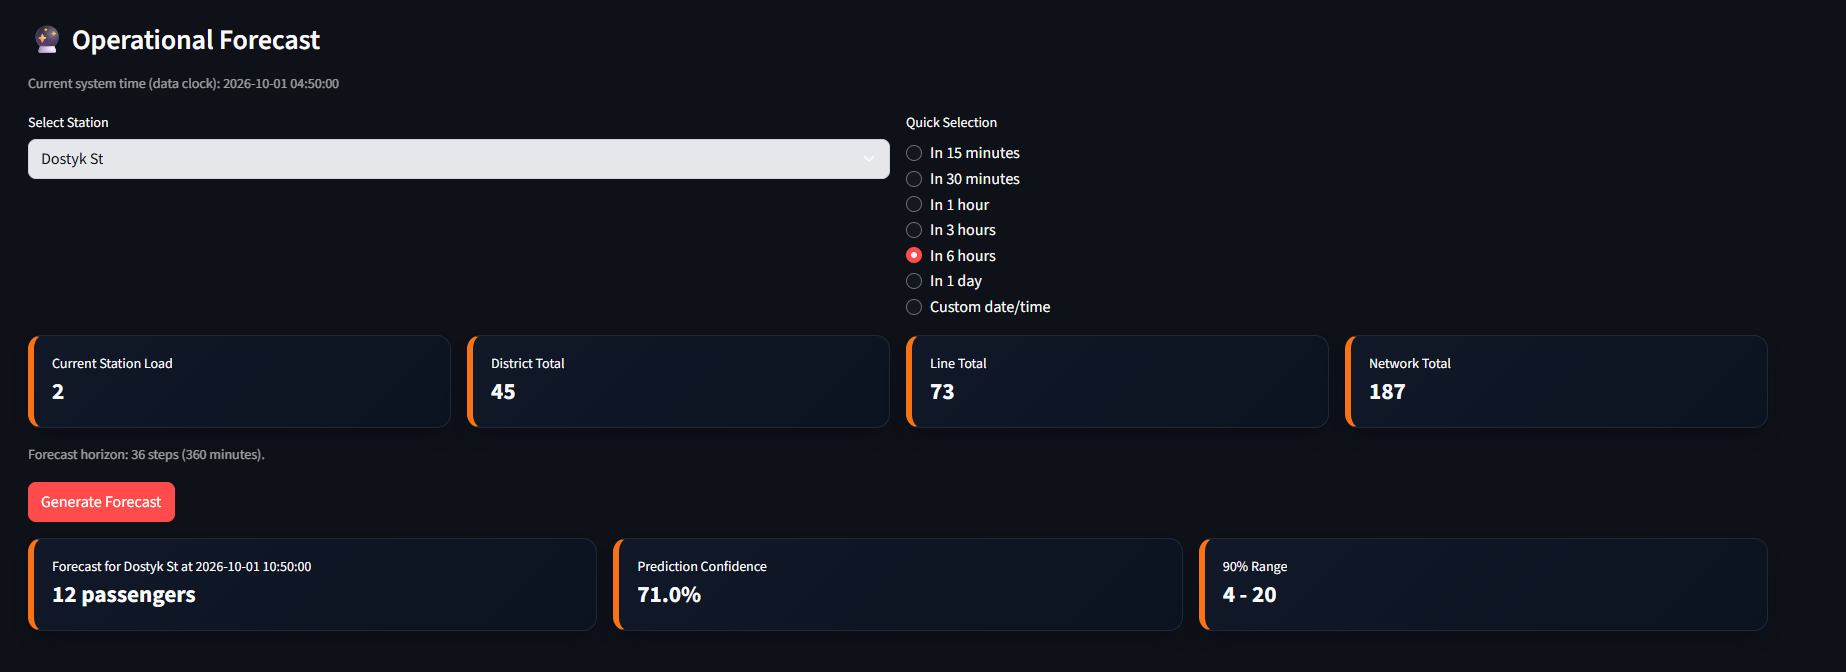
\includegraphics[width=0.95\textwidth]{chapters/methodology/fig/streamlit-operational-forecast-of-station-in-time.png}
\caption{Operational forecast view for a single station, showing predicted boarding counts with confidence intervals across multiple horizons.}
\label{Fig.streamlit_forecast}
\end{figure}

\begin{figure}[H]
\centering
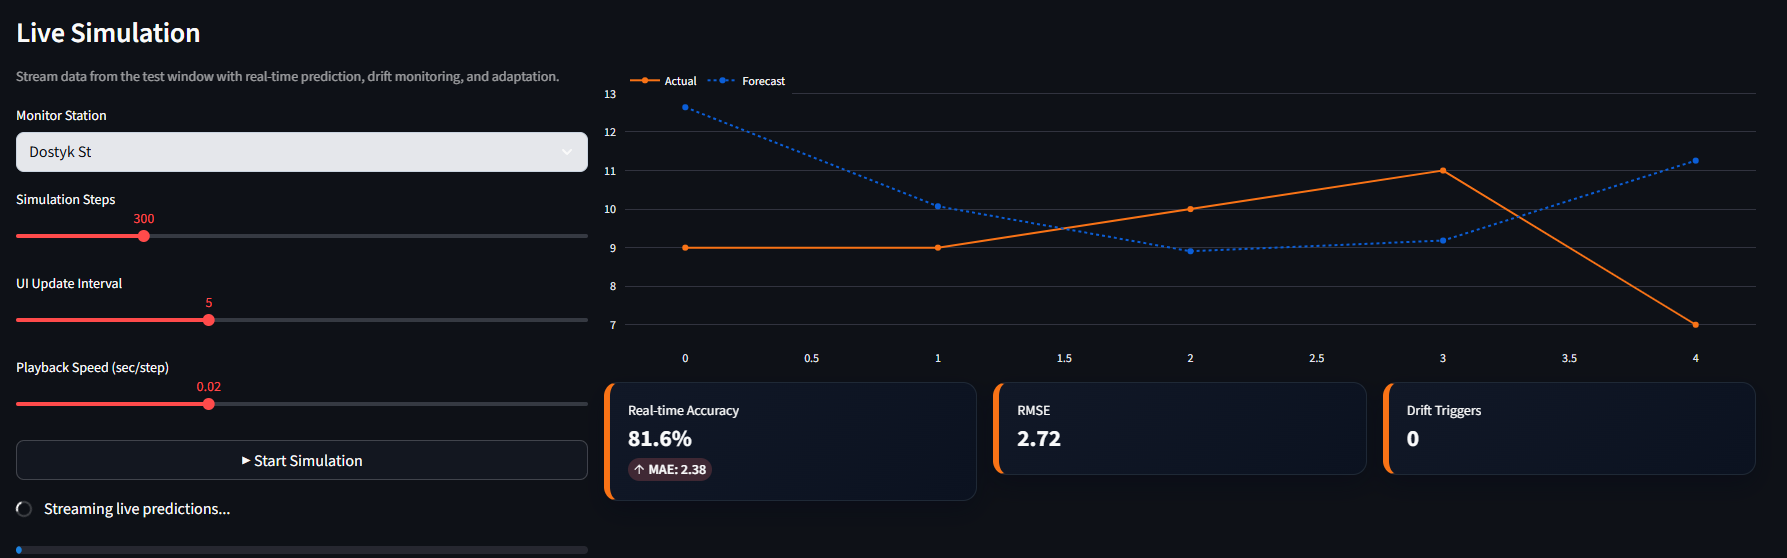
\includegraphics[width=0.95\textwidth]{chapters/methodology/fig/streamlit-live-simulation-of-realtime-data-and-validation.png}
\caption{Streamlit interface for live simulation of real-time data ingestion and model validation. The panel displays incoming ridership observations alongside predicted values and confidence intervals.}
\label{Fig.streamlit_validation}
\end{figure}

\begin{table}[H]
\centering
\caption{Complete training and model hyperparameters.}
\label{Tab.hyperparams}
\begin{tabular}{ll}
\toprule
Parameter & Value \\
\midrule
Context window $T$ & 72 hours \\
Prediction horizons $H_{\text{pred}}$ & 4 (15/30/60/120 min) \\
Input features $F$ & 16 \\
Model dimension $d_{\text{model}}$ & 192 \\
LoRA rank $r$ & 16 \\
Attention heads $n_h$ & 6 \\
Graph hops $K$ & 3 \\
Adjacency mixing $\alpha$ & learnable ($\alpha_0 = 0.6$) \\
Learning rate & $3 \times 10^{-4}$ \\
Weight decay & $10^{-3}$ \\
Warmup epochs & 20 \\
LR scheduler & CosineAnnealing \\
Batch size (effective) & 32 (8 $\times$ 4 accum) \\
Gradient clipping & max\_norm $= 1.0$ \\
Mixed precision & FP16 (CUDA) \\
Dropout & 0.1 \\
Early stopping patience & 50 epochs \\
Max training epochs & 500 \\
Train/Val/Test split & 70\% / 15\% / 15\% \\
Trainable parameters & 469{,}697 \\
\bottomrule
\end{tabular}
\end{table}

Several hyperparameters warrant justification. The context window $T = 72$ hours captures three full daily cycles, providing the model with sufficient history to learn both diurnal and day-of-week patterns while remaining tractable for the $O(T^2)$ attention mechanism. The model dimension $d_{\text{model}} = 192$ balances expressiveness against overfitting on a dataset of 1.3 million records; smaller dimensions ($d = 64, 128$) underfit the spatial structure, while larger values ($d = 256$) yield diminishing validation $R^2$ gains ($< 0.2\%$) at twice the memory cost. The LoRA rank $r = 16$ and scaling $\alpha = 16$ follow the configuration recommended by Hu et al.\ \cite{hu2022lora}, yielding a rank-to-dimension ratio of $r/d \approx 0.08$ that preserves fine-tuning capacity while reducing trainable parameters by 94\%. The 6-head attention configuration ($n_h = 6$, $d_h = 32$) provides sufficient capacity for multi-scale temporal patterns; ablation showed that reducing to 4 heads drops $R^2$ by 0.4\%, while 8 heads provides no significant improvement. The auxiliary loss weight $\lambda = 0.3$ was selected from a grid search over $\{0.1, 0.2, 0.3, 0.4, 0.5\}$; values below 0.2 produce unstable training, while values above 0.4 suppress the NB likelihood term and degrade calibration. Gradient clipping (max norm 1.0) prevents exploding gradients in the attention layer, and cosine annealing with warmup provides stable convergence without the sharp restarts of cyclical schedulers.
